The executable {\ttfamily doxygen} is the main program that parses the sources and generates the documentation. See section \hyperlink{doxygen_usage}{Doxygen usage} for more detailed usage information.

The executable {\ttfamily doxytag} is only needed if you want to generate references to external documentation (i.e. documentation that was generated by doxygen) for which you do not have the sources. See section \hyperlink{doxytag_usage}{Doxytag usage} for more detailed usage information.

Optionally, the executable {\ttfamily doxywizard} can be used, which is a \hyperlink{doxywizard_usage}{graphical front-\/end} for editing the configuration file that is used by doxygen and for running doxygen in a graphical environment. For Mac OS X doxywizard will be started by clicking on the Doxygen application icon.

The following figure shows the relation between the tools and the flow of information between them (it looks complex but that's only because it tries to be complete):

 
\begin{DoxyImage}
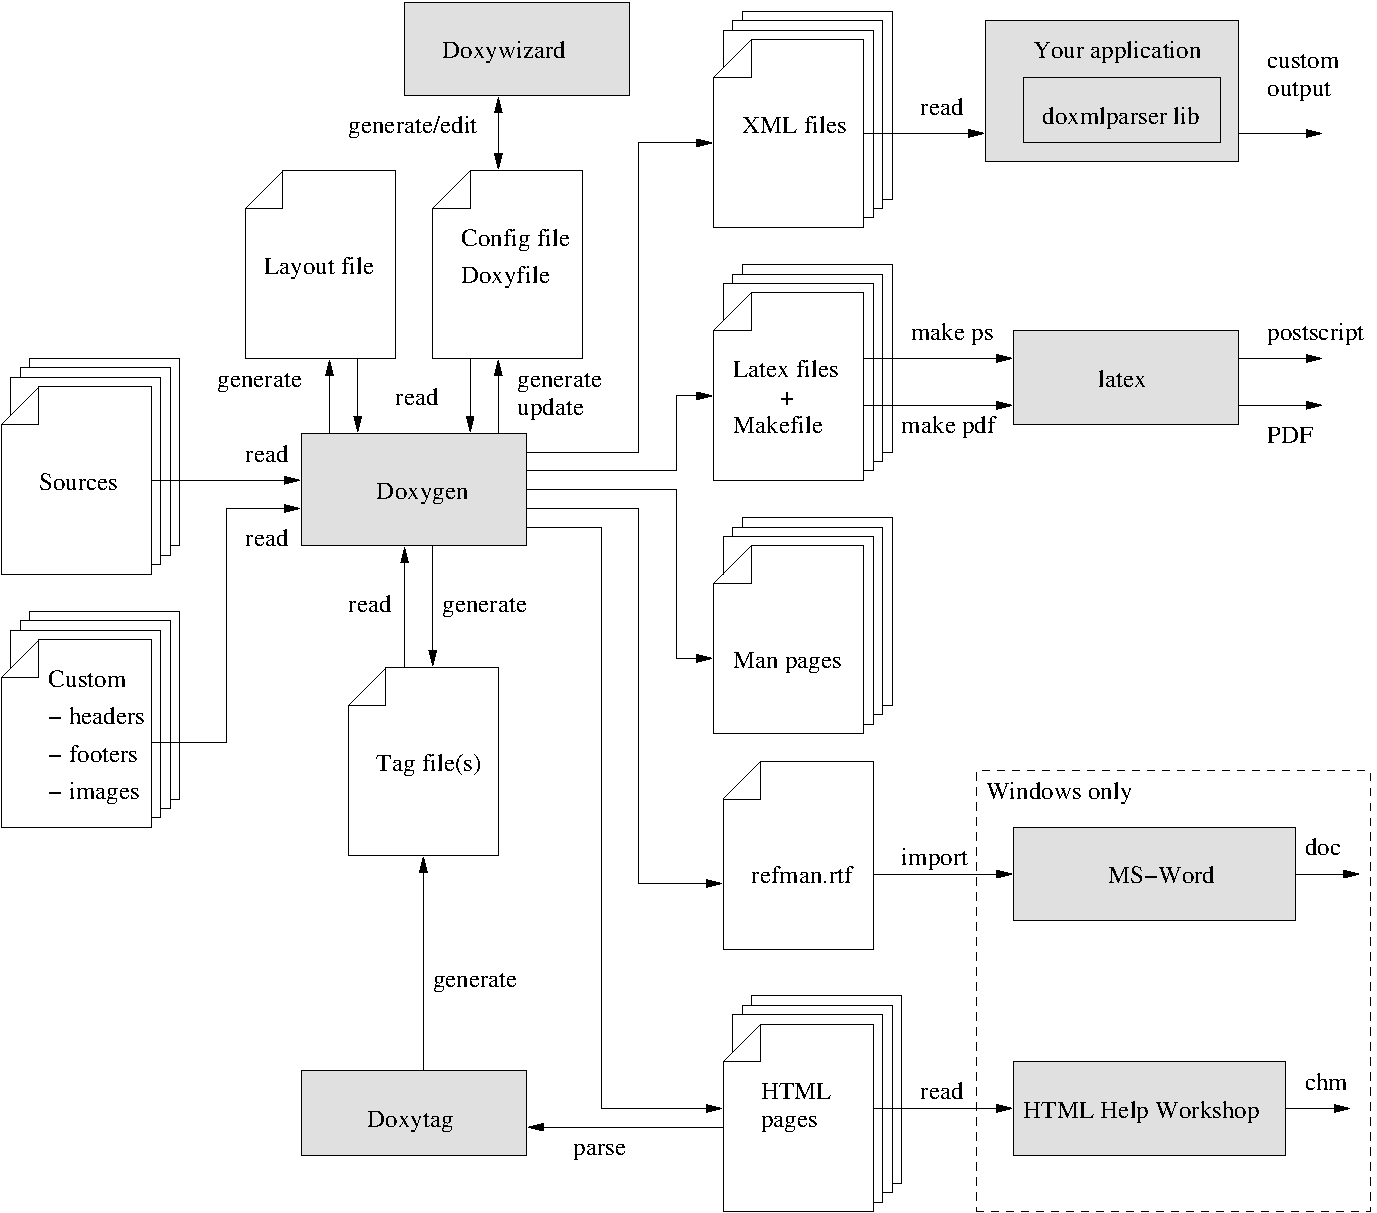
\includegraphics[width=14cm]{infoflow}
\caption{Doxygen information flow}
\end{DoxyImage}
\hypertarget{starting_step1}{}\section{Step 1: Creating a configuration file}\label{starting_step1}
Doxygen uses a configuration file to determine all of its settings. Each project should get its own configuration file. A project can consist of a single source file, but can also be an entire source tree that is recursively scanned.

To simplify the creation of a configuration file, doxygen can create a template configuration file for you. To do this call {\ttfamily doxygen} from the command line with the {\ttfamily -\/g} option: \begin{DoxyVerb}
doxygen -g <config-file>
\end{DoxyVerb}


where $<$config-\/file$>$ is the name of the configuration file. If you omit the file name, a file named {\ttfamily Doxyfile} will be created. If a file with the name $<$config-\/file$>$ already exists, doxygen will rename it to $<$config-\/file$>$.bak before generating the configuration template. If you use {\ttfamily -\/} (i.e. the minus sign) as the file name then doxygen will try to read the configuration file from standard input ({\ttfamily stdin}), which can be useful for scripting.

The configuration file has a format that is similar to that of a (simple) Makefile. It consists of a number of assignments (tags) of the form:

{\ttfamily TAGNAME = VALUE} or \par
 {\ttfamily TAGNAME = VALUE1 VALUE2 ... }\par


You can probably leave the values of most tags in a generated template configuration file to their default value. See section \hyperlink{config}{Configuration} for more details about the configuration file.

If you do not wish to edit the config file with a text editor, you should have a look at \hyperlink{doxywizard_usage}{doxywizard}, which is a GUI front-\/end that can create, read and write doxygen configuration files, and allows setting configuration options by entering them via dialogs.

For a small project consisting of a few C and/or C++ source and header files, you can leave \hyperlink{config_cfg_input}{INPUT} tag empty and doxygen will search for sources in the current directory.

If you have a larger project consisting of a source directory or tree you should assign the root directory or directories to the \hyperlink{config_cfg_input}{INPUT} tag, and add one or more file patterns to the \hyperlink{config_cfg_file_patterns}{FILE\_\-PATTERNS} tag (for instance {\ttfamily $\ast$.cpp $\ast$.h}). Only files that match one of the patterns will be parsed (if the patterns are omitted a list of source extensions is used). For recursive parsing of a source tree you must set the \hyperlink{config_cfg_recursive}{RECURSIVE} tag to {\ttfamily YES}. To further fine-\/tune the list of files that is parsed the \hyperlink{config_cfg_exclude}{EXCLUDE} and \hyperlink{config_cfg_exclude_patterns}{EXCLUDE\_\-PATTERNS} tags can be used. To omit all {\ttfamily test} directories from a source tree for instance, one could use: \begin{DoxyVerb}EXCLUDE_PATTERNS = */test/* 
\end{DoxyVerb}


Doxygen looks at the file's extension to determine how to parse a file. If a file has an {\ttfamily .idl} or {\ttfamily .odl} extension it is treated as an IDL file. If it has a {\ttfamily .java} extension it is treated as a file written in Java. Files ending with {\ttfamily .cs} are treated as C\# files and the {\ttfamily .py} extension selects the Python parser. Finally, files with the extensions {\ttfamily .php}, {\ttfamily .php4}, {\ttfamily .inc} or {\ttfamily .phtml} are treated as PHP sources. Any other extension is parsed as if it is a C/C++ file, where files that end with {\ttfamily .m} are treated as Objective-\/C source files.

\label{starting_extract_all}
\hypertarget{starting_extract_all}{}
 If you start using doxygen for an existing project (thus without any documentation that doxygen is aware of), you can still get an idea of what the structure is and how the documented result would look like. To do so, you must set the \hyperlink{config_cfg_extract_all}{EXTRACT\_\-ALL} tag in the configuration file to {\ttfamily YES}. Then, doxygen will pretend everything in your sources is documented. Please note that as a consequence warnings about undocumented members will not be generated as long as \hyperlink{config_cfg_extract_all}{EXTRACT\_\-ALL} is set to {\ttfamily YES}.

To analyse an existing piece of software it is useful to cross-\/reference a (documented) entity with its definition in the source files. Doxygen will generate such cross-\/references if you set the \hyperlink{config_cfg_source_browser}{SOURCE\_\-BROWSER} tag to {\ttfamily YES}. It can also include the sources directly into the documentation by setting \hyperlink{config_cfg_inline_sources}{INLINE\_\-SOURCES} to {\ttfamily YES} (this can be handy for code reviews for instance).\hypertarget{starting_step2}{}\section{Step 2: Running doxygen}\label{starting_step2}
To generate the documentation you can now enter: \begin{DoxyVerb}
doxygen <config-file>
\end{DoxyVerb}


Depending on your settings doxygen will create {\ttfamily html}, {\ttfamily rtf}, {\ttfamily latex}, {\ttfamily xml} and/or {\ttfamily man} directories inside the output directory. As the names suggest these directories contain the generated documentation in HTML, RTF, $\mbox{\LaTeX}$, XML and Unix-\/Man page format.

The default output directory is the directory in which {\ttfamily doxygen} is started. The root directory to which the output is written can be changed using the \hyperlink{config_cfg_output_directory}{OUTPUT\_\-DIRECTORY}. The format specific directory within the output directory can be selected using the \hyperlink{config_cfg_html_output}{HTML\_\-OUTPUT}, \hyperlink{config_cfg_rtf_output}{RTF\_\-OUTPUT}, \hyperlink{config_cfg_latex_output}{LATEX\_\-OUTPUT}, \hyperlink{config_cfg_xml_output}{XML\_\-OUTPUT}, and \hyperlink{config_cfg_man_output}{MAN\_\-OUTPUT} tags of the configuration file. If the output directory does not exist, {\ttfamily doxygen} will try to create it for you (but it will {\itshape not\/} try to create a whole path recursively, like {\ttfamily mkdir -\/p} does).\hypertarget{starting_html_out}{}\subsection{HTML output}\label{starting_html_out}
\index{browser@{browser}} The generated HTML documentation can be viewed by pointing a HTML browser to the {\ttfamily index.html} file in the {\ttfamily html} directory. For the best results a browser that supports cascading style sheets (CSS) should be used (I'm using Mozilla, Safari, Konqueror, and sometimes IE6 to test the generated output).

Some of the features the HTML section (such as \hyperlink{config_cfg_generate_treeview}{GENERATE\_\-TREEVIEW} or the search engine) require a browser that supports DHTML and Javascript.\hypertarget{starting_latex_out}{}\subsection{LaTeX output}\label{starting_latex_out}
\index{LaTeX@{LaTeX}} The generated $\mbox{\LaTeX}$ documentation must first be compiled by a $\mbox{\LaTeX}$ compiler (I use a recent teTeX distribution). To simplify the process of compiling the generated documentation, {\ttfamily doxygen} writes a {\ttfamily Makefile} into the {\ttfamily latex} directory.

The contents and targets in the {\ttfamily Makefile} depend on the setting of \hyperlink{config_cfg_use_pdflatex}{USE\_\-PDFLATEX}. If it is disabled (set to {\ttfamily NO}), then typing {\ttfamily make} in the {\ttfamily latex} directory a dvi file called {\ttfamily refman.dvi} will be generated. This file can then be viewed using {\ttfamily xdvi} or converted into a PostScript file {\ttfamily refman.ps} by typing {\ttfamily make ps} (this requires {\ttfamily dvips}).

To put 2 pages on one physical page use {\ttfamily make ps\_\-2on1} instead. The resulting PostScript file can be send to a PostScript printer. If you do not have a PostScript printer, you can try to use ghostscript to convert PostScript into something your printer understands.

Conversion to PDF is also possible if you have installed the ghostscript interpreter; just type {\ttfamily make pdf} (or {\ttfamily make pdf\_\-2on1}).

To get the best results for PDF output you should set the \hyperlink{config_cfg_pdf_hyperlinks}{PDF\_\-HYPERLINKS} and \hyperlink{config_cfg_use_pdflatex}{USE\_\-PDFLATEX} tags to {\ttfamily YES}. In this case the {\ttfamily Makefile} will only contain a target to build {\ttfamily refman.pdf} directly.\hypertarget{starting_rtf_out}{}\subsection{RTF output}\label{starting_rtf_out}
\index{RTF@{RTF}} Doxygen combines the RTF output to a single file called refman.rtf. This file is optimized for importing into the Microsoft Word. Certain information is encoded using field. To show the actual value you need to select all (Edit -\/ select all) and then toggle fields (right click and select the option from the drop down menu).\hypertarget{starting_xml_out}{}\subsection{XML output}\label{starting_xml_out}
\index{XML@{XML}} The XML output consists of a structured \char`\"{}dump\char`\"{} of the information gathered by doxygen. Each compound (class/namespace/file/...) has its own XML file and there is also an index file called index.xml.

A file called combine.xslt XSLT script is also generated and can be used to combine all XML files into a single file.

Doxygen also generates two XML schema files index.xsd (for the index file) and compound.xsd (for the compound files). This schema file describes the possible elements, their attributes and how they are structured, i.e. it the describes the grammar of the XML files and can be used for validation or to steer XSLT scripts.

In the addon/doxmlparser directory you can find a parser library for reading the XML output produced by doxygen in an incremental way (see addon/doxmlparser/include/doxmlintf.h for the interface of the library)\hypertarget{starting_man_out}{}\subsection{Man page output}\label{starting_man_out}
The generated man pages can be viewed using the {\ttfamily man} program. You do need to make sure the man directory is in the man path (see the {\ttfamily MANPATH} environment variable). Note that there are some limitations to the capabilities of the man page format, so some information (like class diagrams, cross references and formulas) will be lost.\hypertarget{starting_step3}{}\section{Step 3: Documenting the sources}\label{starting_step3}
Although documenting the sources is presented as step 3, in a new project this should of course be step 1. Here I assume you already have some code and you want doxygen to generate a nice document describing the API and maybe the internals as well.

If the \hyperlink{config_cfg_extract_all}{EXTRACT\_\-ALL} option is set to {\ttfamily NO} in the configuration file (the default), then doxygen will only generate documentation for {\itshape documented\/} members, files, classes and namespaces. So how do you document these? For members, classes and namespaces there are basically two options: 
\begin{DoxyEnumerate}
\item Place a {\itshape special\/} documentation block in front of the declaration or definition of the member, class or namespace. For file, class and namespace members it is also allowed to place the documention directly after the member. See section \hyperlink{docblocks_specialblock}{Special documentation blocks} to learn more about special documentation blocks. 
\item Place a special documentation block somewhere else (another file or another location) {\itshape and\/} put a {\itshape structural command\/} in the documentation block. A structural command links a documentation block to a certain entity that can be documented (e.g. a member, class, namespace or file). See section \hyperlink{docblocks_structuralcommands}{Documentation at other places} to learn more about structural commands. 
\end{DoxyEnumerate}Files can only be documented using the second option, since there is no way to put a documentation block before a file. Of course, file members (functions, variable, typedefs, defines) do not need an explicit structural command; just putting a special documentation block in front or behind them will do.

The text inside a special documentation block is parsed before it is written to the HTML and/or $\mbox{\LaTeX}$ output files.

\index{parsing@{parsing}} During parsing the following steps take place: 
\begin{DoxyItemize}
\item The special commands inside the documentation are executed. See section \hyperlink{commands}{Special Commands} for an overview of all commands. 
\item If a line starts with some whitespace followed by one or more asterisks ({\ttfamily $\ast$}) and then optionally more whitespace, then all whitespace and asterisks are removed. 
\item All resulting blank lines are treated as a paragraph separators. This saves you from placing new-\/paragraph commands yourself in order to make the generated documentation readable. 
\item Links are created for words corresponding to documented classes (unless the word is preceded by a \%; then the word will not be linked and the \% sign is removed). 
\item Links to members are created when certain patterns are found in the text. See section \hyperlink{autolink}{Automatic link generation} for more information on how the automatic link generation works. 
\item HTML tags that are in the documentation are interpreted and converted to $\mbox{\LaTeX}$ equivalents for the $\mbox{\LaTeX}$ output. See section \hyperlink{htmlcmds}{HTML Commands} for an overview of all supported HTML tags. 
\end{DoxyItemize}

 